\documentclass[tikz]{standalone}

\usetikzlibrary{calc, intersections}

\colorlet{FilledSurface}{blue!20}
\colorlet{FilledSurfaceGroupOne}{blue!20}
\colorlet{FilledSurfaceGroupTwo}{red!20}
\colorlet{FilledSurfaceGroupThree}{green!20}
\colorlet{FilledSurfaceGroupFour}{magenta!20}
\colorlet{FormulaBackground}{green!10}
\colorlet{FormulaFrame}{green}


\begin{document}
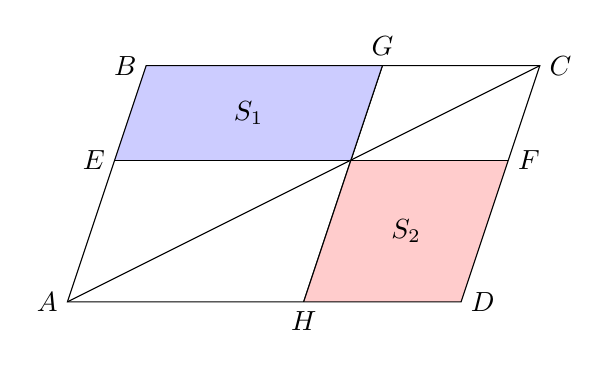
\begin{tikzpicture}

    \coordinate (A) at (0, 0);
    \coordinate (B) at (1, 3);
    \coordinate (C) at (6, 3);
    \coordinate (D) at (5, 0);

    % Punto arbitrario paralelos en lados opuestos AB y CD
    \coordinate (E) at ($(A)!0.6!(B)$);
    \coordinate (F) at ($(D)!0.6!(C)$);

    % Punto arbitrario paralelos en lados opuestos BC y AD
    \coordinate (G) at ($(B)!0.6!(C)$);
    \coordinate (H) at ($(A)!0.6!(D)$);

    \draw[name path=EF] (E) -- (F);
    \draw[name path=GH] (G) -- (H);
    \path [name intersections={of=EF and GH, by=I}];

    \fill[FilledSurfaceGroupOne] (B) -- (G) -- (I) -- (E);
    \fill[FilledSurfaceGroupTwo] (D) -- (H) -- (I) -- (F);

    \draw
    (A) node[left] {$A$}
    -- (B) node [left] {$B$}
    -- (C) node [right] {$C$}
    -- (D) node [right] {$D$}
    -- cycle;
    \draw (E) node [left] {$E$} -- (F) node [right] {$F$};
    \draw (G) node [above] {$G$} -- (H) node [below] {$H$};
    \draw (A) -- (C);

    \node at (barycentric cs:B=1,G=1,I=1,E=1) {$S_1$};
    \node at (barycentric cs:D=1,H=1,I=1,F=1) {$S_2$};
\end{tikzpicture}
\end{document}
